\documentclass{article}
\usepackage[UTF8, scheme = plain]{ctex}
\usepackage{amsmath,amsfonts,amsthm,amssymb,amssymb,amsfonts}
\usepackage{setspace}
\usepackage{fancyhdr}
\usepackage{lastpage}
\usepackage{extramarks}
\usepackage{chngpage}
\usepackage{soul,color}
\usepackage{graphicx,float,wrapfig}
\usepackage{CJKutf8}
\usepackage{graphicx}
\usepackage[noend]{algpseudocode}
\usepackage{algorithmicx,algorithm}
\usepackage{listings}
\usepackage{subfigure}
\newcommand{\Class}{人工智能导论}
%\newcommand{\ClassInstructor}{Jian Li}%

% Homework Specific Information. Change it to your own
\newcommand{\Title}{文本情感分类器}
%\newcommand{\DueDate}{Oct 12, 2022}
\newcommand{\StudentName}{周韧平}
\newcommand{\StudentClass}{计 11}
\newcommand{\StudentNumber}{2021010699}

% In case you need to adjust margins:
\topmargin=-0.45in      %
\evensidemargin=0in     %
\oddsidemargin=0in      %
\textwidth=6.5in        %
\textheight=9.0in       %
\headsep=0.25in         %

% Setup the header and footer
\pagestyle{fancy}                                                       %
\lhead{\StudentName}                                                 %
\chead{\Title}  %
\rhead{\firstxmark}                                                     %
\lfoot{\lastxmark}                                                      %
\cfoot{}                                                                %
\rfoot{Page\ \thepage\ of\ \protect\pageref{LastPage}}                          %
\renewcommand\headrulewidth{0.4pt}                                      %
\renewcommand\footrulewidth{0.4pt}                                      %

%%%%%%%%%%%%%%%%%%%%%%%%%%%%%%%%%%%%%%%%%%%%%%%%%%%%%%%%%%%%%
% Some tools
\newcommand{\enterProblemHeader}[1]{\nobreak\extramarks{#1}{#1 continued on next page\ldots}\nobreak%
                                    \nobreak\extramarks{#1 (continued)}{#1 continued on next page\ldots}\nobreak}%
\newcommand{\exitProblemHeader}[1]{\nobreak\extramarks{#1 (continued)}{#1 continued on next page\ldots}\nobreak%
                                   \nobreak\extramarks{#1}{}\nobreak}%

\newcommand{\homeworkProblemName}{}%
\newcounter{homeworkProblemCounter}%
\newenvironment{homeworkProblem}[1][Problem \arabic{homeworkProblemCounter}]%
  {\stepcounter{homeworkProblemCounter}%
   \renewcommand{\homeworkProblemName}{#1}%
   \section*{\homeworkProblemName}%
   \enterProblemHeader{\homeworkProblemName}}%
  {\exitProblemHeader{\homeworkProblemName}}%

\newcommand{\homeworkSectionName}{}%
\newlength{\homeworkSectionLabelLength}{}%
\newenvironment{homeworkSection}[1]%
  {% We put this space here to make sure we're not connected to the above.

   \renewcommand{\homeworkSectionName}{#1}%
   \settowidth{\homeworkSectionLabelLength}{\homeworkSectionName}%
   \addtolength{\homeworkSectionLabelLength}{0.25in}%
   \changetext{}{-\homeworkSectionLabelLength}{}{}{}%
   \subsection*{\homeworkSectionName}%
   \enterProblemHeader{\homeworkProblemName\ [\homeworkSectionName]}}%
  {\enterProblemHeader{\homeworkProblemName}%

   % We put the blank space above in order to make sure this margin
   % change doesn't happen too soon.
   \changetext{}{+\homeworkSectionLabelLength}{}{}{}}%

\newcommand{\Answer}{\ \\\textbf{Answer:} }
\newcommand{\Proof}{\ \\\textbf{Proof:} }
\newcommand{\Acknowledgement}[1]{\ \\{\bf Acknowledgement:} #1}
\newcommand{\D}{\text{ d}}

%%%%%%%%%%%%%%%%%%%%%%%%%%%%%%%%%%%%%%%%%%%%%%%%%%%%%%%%%%%%%
\lstset{ %
	language=C++,                % choose the language of the code
	basicstyle=\fontspec{Consolas},       % the size of the fonts that are used for the code
	%numbers=left,                   % where to put the line-numbers
	numberstyle=\footnotesize,      % the size of the fonts that are used for the line-numbers
	stepnumber=1,                   % the step between two line-numbers. If it is 1 each line will be numbered
	numbersep=5pt,                  % how far the line-numbers are from the code
	backgroundcolor=\color{white},  % choose the background color. You must add \usepackage{color}
	showspaces=false,               % show spaces adding particular underscores
	showstringspaces=false,         % underline spaces within strings
	showtabs=false,                 % show tabs within strings adding particular underscores
	frame=single,           % adds a frame around the code
	tabsize=2,          % sets default tabsize to 2 spaces
	captionpos=b,           % sets the caption-position to bottom
	breaklines=true,        % sets automatic line breaking
	breakatwhitespace=false,    % sets if automatic breaks should only happen at whitespace
	escapeinside={\%*}{*)}          % if you want to add a comment within your code
}

%%%%%%%%%%%%%%%%%%%%%%%%%%%%%%%%%%%%%%%%%%%%%%%%%%%%%%%%%%%%%
% Make title
\title{\textmd{\bf \Class: \Title}}
\author{\textbf{\StudentName}\ \ \StudentClass\ \ \StudentNumber}
%%%%%%%%%%%%%%%%%%%%%%%%%%%%%%%%%%%%%%%%%%%%%%%%%%%%%%%%%%%%%

\begin{document}
\begin{spacing}{1.1}
\maketitle \thispagestyle{empty}
%\cite{}
%%%%%%%%%%%%%%%%%%%%%%%%%%%%%%%%%%%%%%%%%%%%%%%%%%%%%%%%%%%%%
% Begin edit from here
\section{摘要}
\hspace{1.4em} 本次实验中,我尝试用 pytorch 深度学习框架搭建了 MLP,TextCNN,RNN-LSTM, RNN-GRU 四种模型架构,在给定词向量的情况下,使用给定数据集做了文本情感二分类实验。实验中,我通过调节模型结构和参数初始化等超参数设置并进行多次实验,尝试分析不同参数对实验结果以及训练成本可能造成的影响。代码框架层面,我搭建了具有可扩展性的代码框架,以便于实验和可能未来引入的更多模型。

\section{基本原理}
	\subsection{词向量嵌入模型: Word2Vec}
	\hspace{1.4em} 
	所谓词向量模型就是就是将一个词映射成 $\mathbb{R}^n$ 向量的过程,独热编码(one hot)方法虽然操作简便,但无法准确表达不同词之间的相似性,词向量嵌入的动机就在于此,它通过定长向量来表示词与词之间的相似关系,尝试在向量中蕴含更多的信息。
	
	目前有两种比较成熟的训练 Word2Vec 的方法:词袋模型(CBOW)和跳词模型 Skip-gram,二者共同特点的都是基于在给定窗口内通过词与词出现的频率去学习独热编码到词向量的映射矩阵,不过 skip-gram 模型是用背景词作为“老师”来训练中心词这个“学生”,而 cbow 模型刚好相反,是中心词作为“老师”训练周围词这些“学生”。除此以外,两种模型在损失函数的定义、训练细节等方面也存在差异。其中用到的 Negtive sampling, 背景词和中心词向量表示的方法也在其它模型中被广泛应用。
	 
	关于“嵌入”的含义,我个人的理解是由于独热编码转化到词向量中间乘以矩阵的计算过于复杂,而独热编码本身是一个稀疏矩阵,所以实际操作过程中就是从矩阵中取出对应的行或者列,也就是所谓“嵌入”的含义。
	
	词向量训练并不是本次实验的重点,本次实验中,我使用的是课程作业提供的基于 Wikipidia 训练的 50 维向量模型。
	
	\subsection{模型结构}
	\subsection{MLP 模型}
	\hspace{1.4em} 作为 baseline,MLP模型也是其它模型的基础,其每层之间的转移过程可以表示为公式 $$RELU(X^{i-1}W^{i}+b^{i})$$ 在模型的首部还添加 Embedding 层,用来加载词向量。
	
	
	\begin{figure}[h]
		\centering
		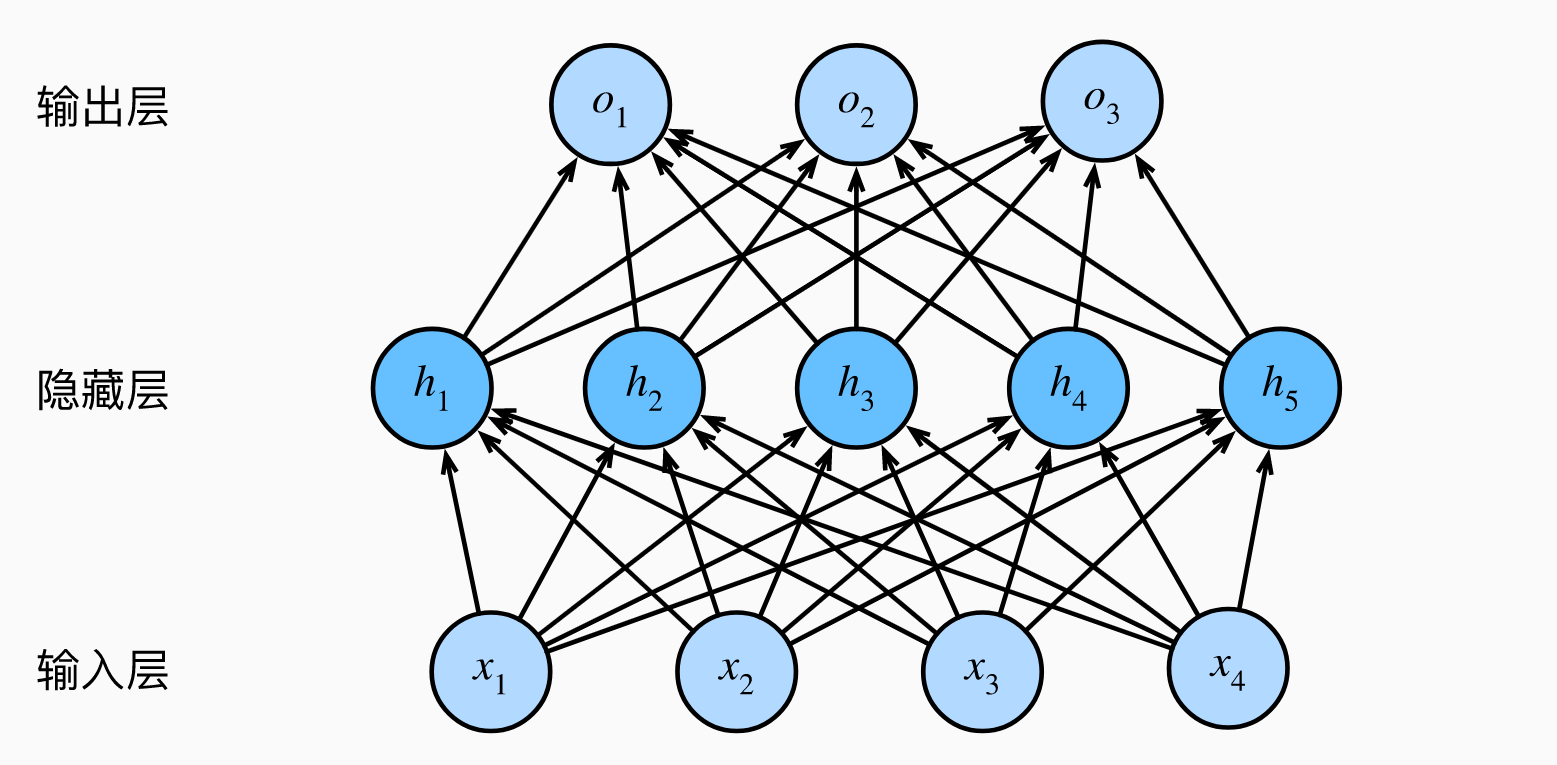
\includegraphics[width=0.8\linewidth]{pic/mlp.png}
		\caption{基本 MLP 模型}
	\end{figure}
	 
	隐藏层可以设计为多层堆叠,实验中我把隐藏层设定为 4-6 层,并在首尾增加了两个 FC 层用来连接输入输出和隐藏层(输入输出的维度分别为 $embedding\_size* length$ 与 $output\_dim$)
	
	\subsection{TextCNN 模型}
	\hspace{1.4em}
	TextCNN模型是一种将卷积神经网络迁移到自然语言处理领域的尝试,它的思想是将词向量按照句子顺序排列成类似图片的形状,然后用一个固定宽度为 embedding size ,长度可选的卷积核去提取句子中的关键信息。和 MLP 类似,TextCNN 模型也在输出层添加了映射到2的 fc 层。上述过程的公式表达为:	
	$$ Output = \sigma(FC(bias + W \times concat\{MaxPool(conv_i(X))\}^{|kernel\_num|}_{i=1})) \ , \ \ X\in M_{embedding\_size\times length} $$
	\begin{figure}[h]
		\centering
		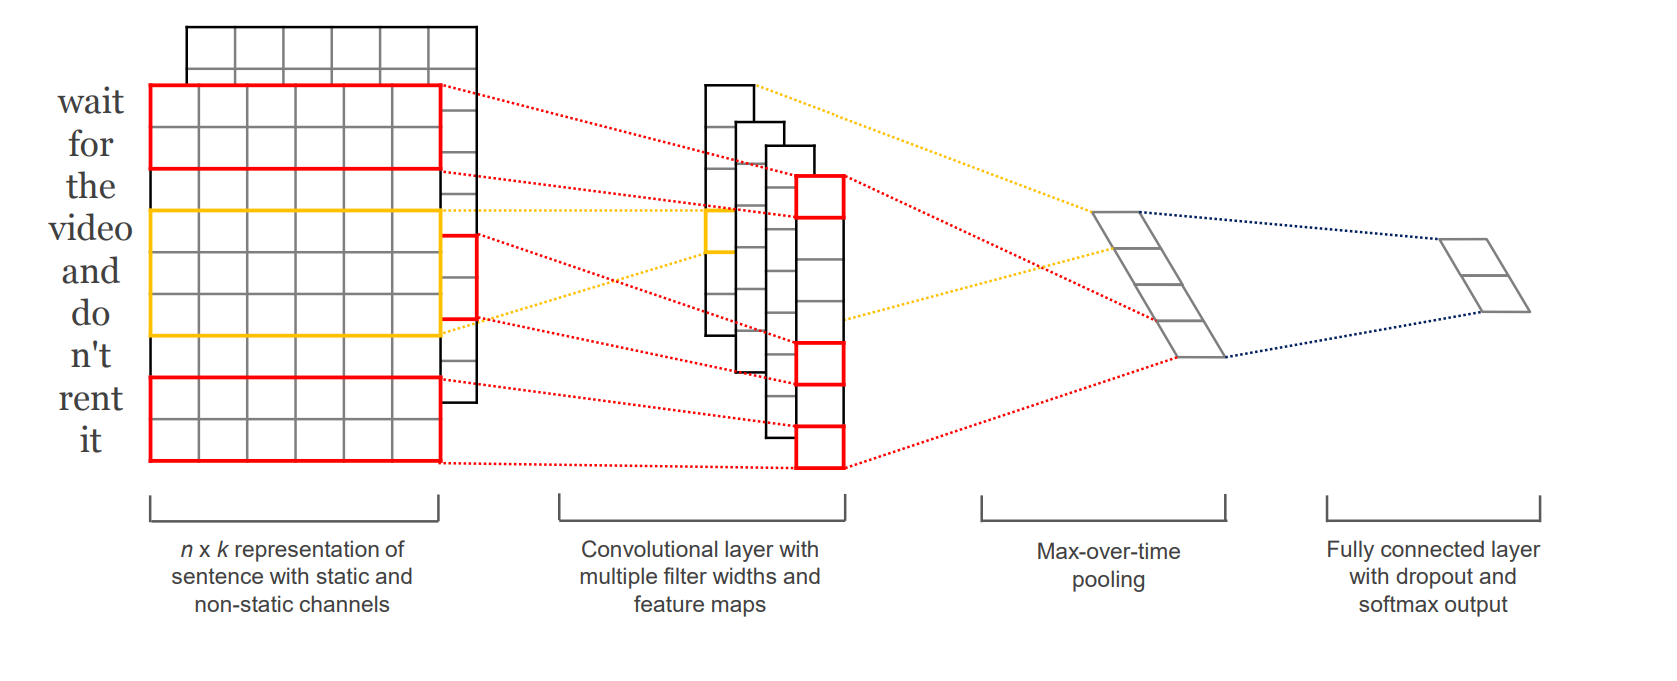
\includegraphics[width=0.8\linewidth]{pic/TextCNN.png}
		\caption{TextCNN 模型}
	\end{figure}
	
	\subsection{RNN-LSTM 模型}
	\hspace{1.4em}
	长短期记忆网络的设计灵感来自于计算机的逻辑门,每一个记忆元 (memory cell)的结构如下图,其中各部分的含义为
	\begin{itemize}
		\item 输入门:决定合适将数据读入单元
		\item 遗忘门:决定重置单元的哪些内容
		\item 输出门:用于从单元中输出条目,产生下一阶段的隐状态
		\item 候选记忆单元:用tanh作为激活函数,影响哪些输入“被记忆”
	\end{itemize}
	
	其公式表示如下
	
	$$
	\begin{aligned}
	 \\ \mathbf{I}_t &= \sigma(\mathbf{X}_t \mathbf{W}_{xi} + \mathbf{H}_{t-1} \mathbf{W}_{hi} + \mathbf{b}_i),
	 \\ \mathbf{F}_t &= \sigma(\mathbf{X}_t \mathbf{W}_{xf} + \mathbf{H}_{t-1} \mathbf{W}_{hf} + \mathbf{b}_f),
	 \\ \mathbf{O}_t &= \sigma(\mathbf{X}_t \mathbf{W}_{xo} + \mathbf{H}_{t-1} \mathbf{W}_{ho} + \mathbf{b}_o),
	 \\ \tilde{\mathbf{C}}_t &= \text{tanh}(\mathbf{X}_t \mathbf{W}_{xc} + \mathbf{H}_{t-1} \mathbf{W}_{hc} + \mathbf{b}_c),
	\end{aligned}
	$$
	
	在定义好门单元后,定义各输出:
	结构如下图,其中各部分的含义为
	\begin{itemize}
		\item 记忆元:遗忘门决定保留上一状态多少信息,输入门决定采用多少输入的信息
		\item 隐状态:将有效的记忆信息传递给下一单元
	\end{itemize}

	公式表示如下
	$$
	\begin{aligned}
	\\ \mathbf{C}_t &= \mathbf{F}_t \odot \mathbf{C}_{t-1} + \mathbf{I}_t \odot \tilde{\mathbf{C}}_t.
	\\ \mathbf{H}_t &= \mathbf{O}_t \odot \tanh(\mathbf{C}_t).
	\end{aligned}
	$$	
	\begin{figure}[h]
		\centering
		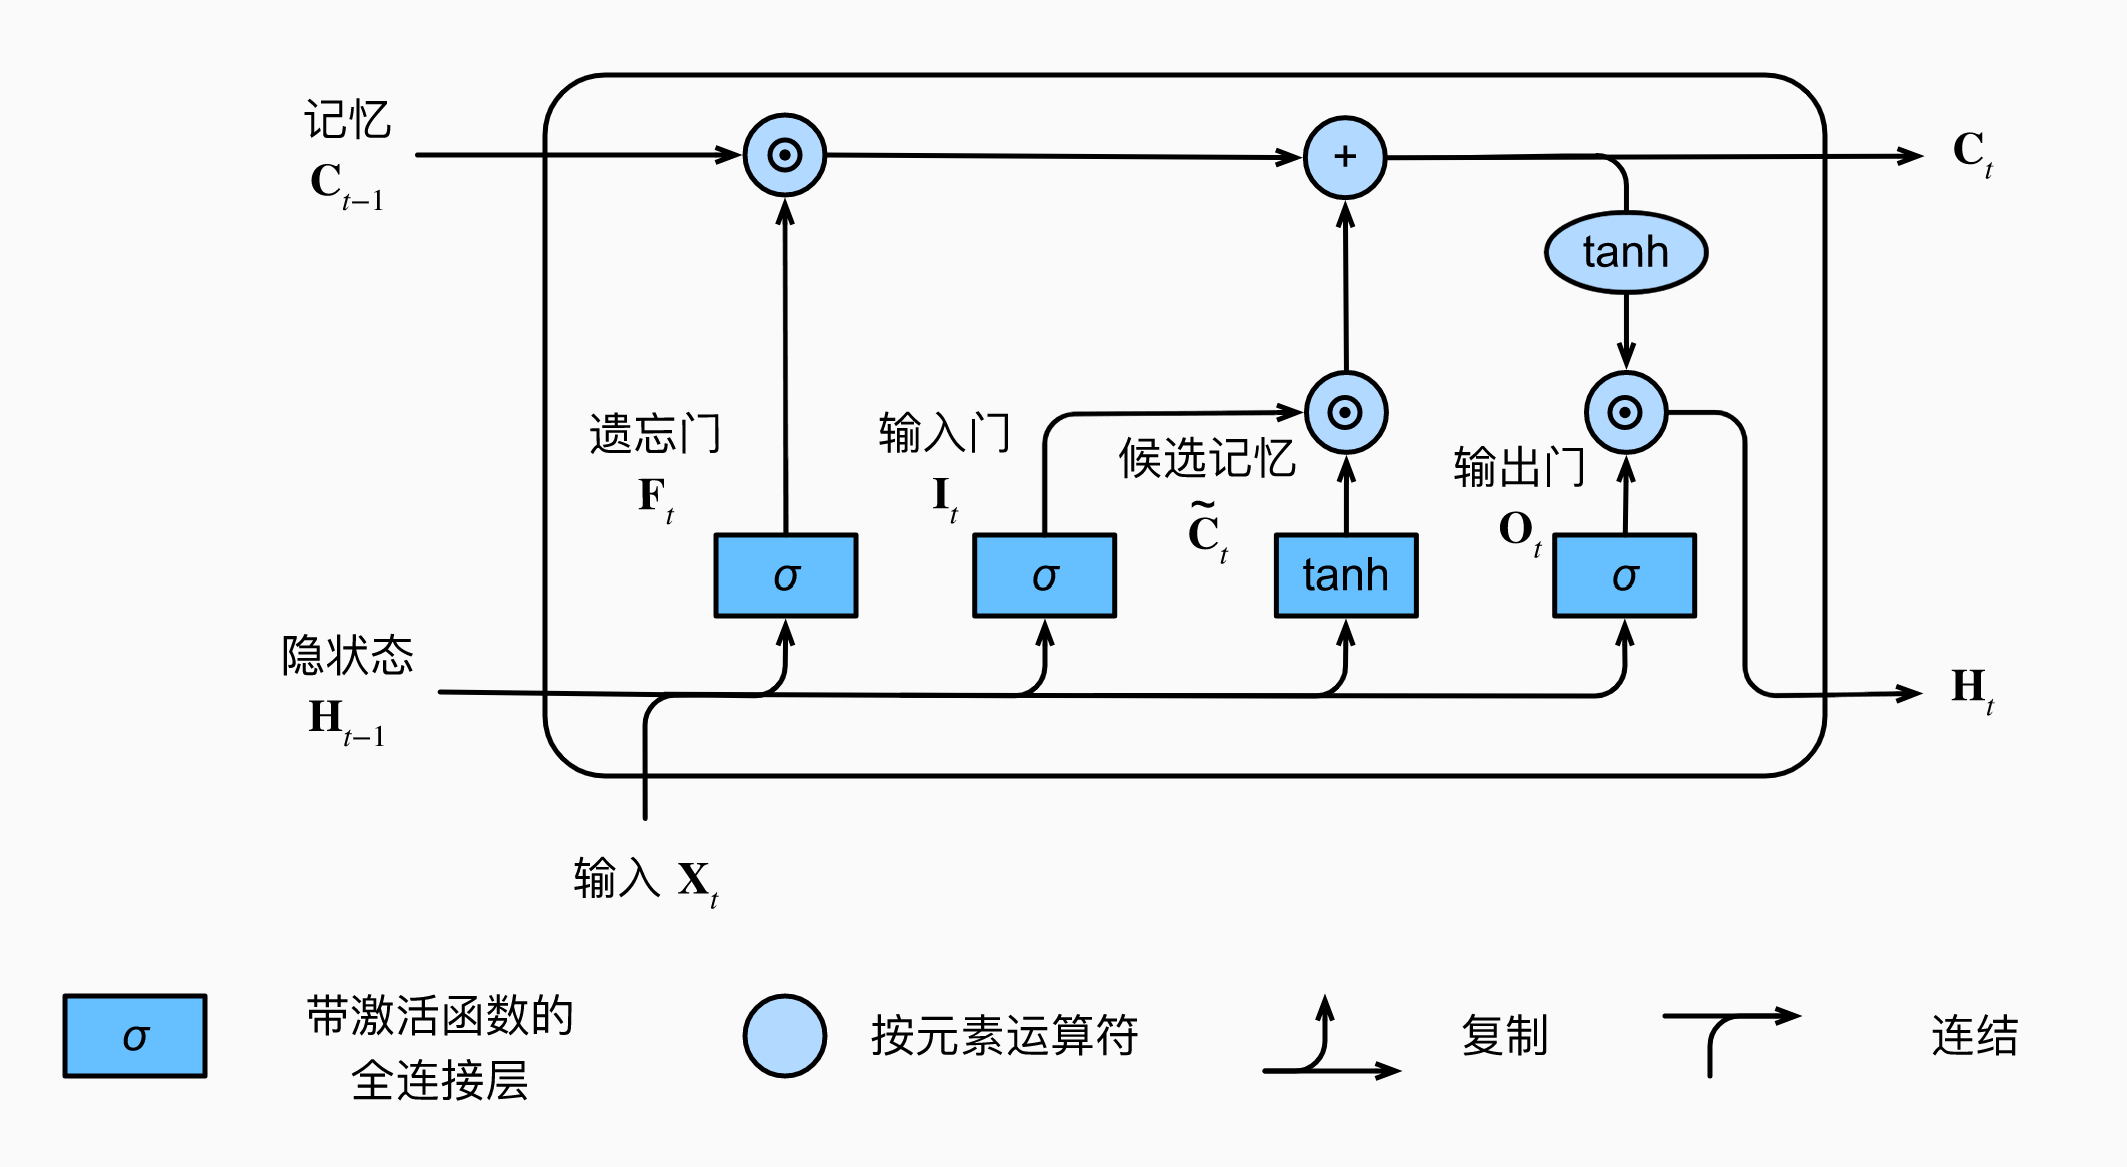
\includegraphics[width=0.8\linewidth]{pic/LSTM.png}
		\caption{LSTM单元}
	\end{figure}
	
	\begin{figure}[h]
		\centering
		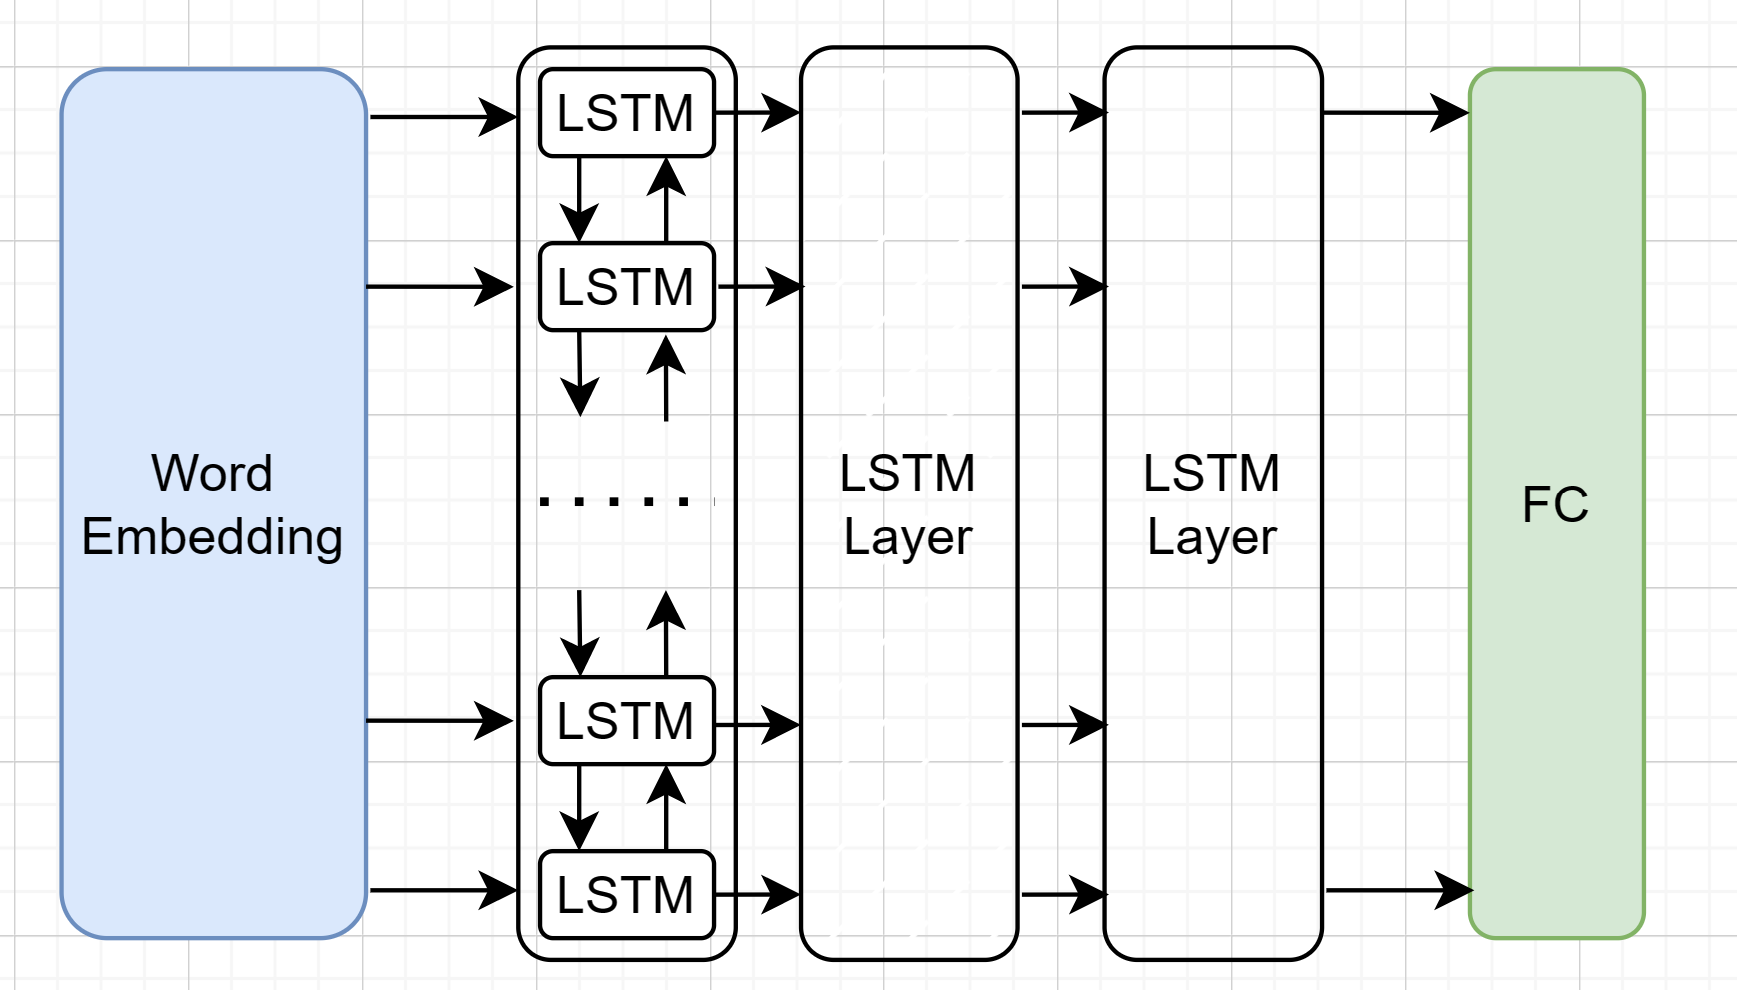
\includegraphics[width=0.8\linewidth]{pic/LSTM-full.png}
		\caption{RNN-LSTM 模型}
	\end{figure}
	
	基于 LSTM 设计的 RNN-LSTM 模型采用双向 LSTM 结构,具体来说,首先经过一层 embedding 层将单词转化成词向量,而后经过 num\_layer 层双向 LSTM,每一层的隐状态输出(首、尾)作为下一层的输入(尾、首),并取最后一层的首尾隐状态输出合并后过 FC 层得到分类结果。
	
	\subsection{RNN-GRU 模型}
	\hspace{1.4em}
	RNN-GRU 模型和基于LSTM的模型相比只是修改了单元结构,重置门有助于捕获序列中的短期依赖关系,更新门有助于捕获序列中的长期依赖关系。其公式表示如下
	$$
	\begin{aligned}
	\mathbf{R}_t &= \sigma(\mathbf{X}_t \mathbf{W}_{xr} + \mathbf{H}_{t-1} \mathbf{W}_{hr} + \mathbf{b}_r),\\
	\mathbf{Z}_t &= \sigma(\mathbf{X}_t \mathbf{W}_{xz} + \mathbf{H}_{t-1} \mathbf{W}_{hz} + \mathbf{b}_z),\\
	\tilde{\mathbf{H}}_t &= \tanh(\mathbf{X}_t \mathbf{W}_{xh} + \left(\mathbf{R}_t \odot \mathbf{H}_{t-1}\right) \mathbf{W}_{hh} + \mathbf{b}_h),\\
	\mathbf{H}_t &= \mathbf{Z}_t \odot \mathbf{H}_{t-1}  + (1 - \mathbf{Z}_t) \odot \tilde{\mathbf{H}}_t.
	\end{aligned}
	$$	
	\begin{figure}[h]
		\centering
		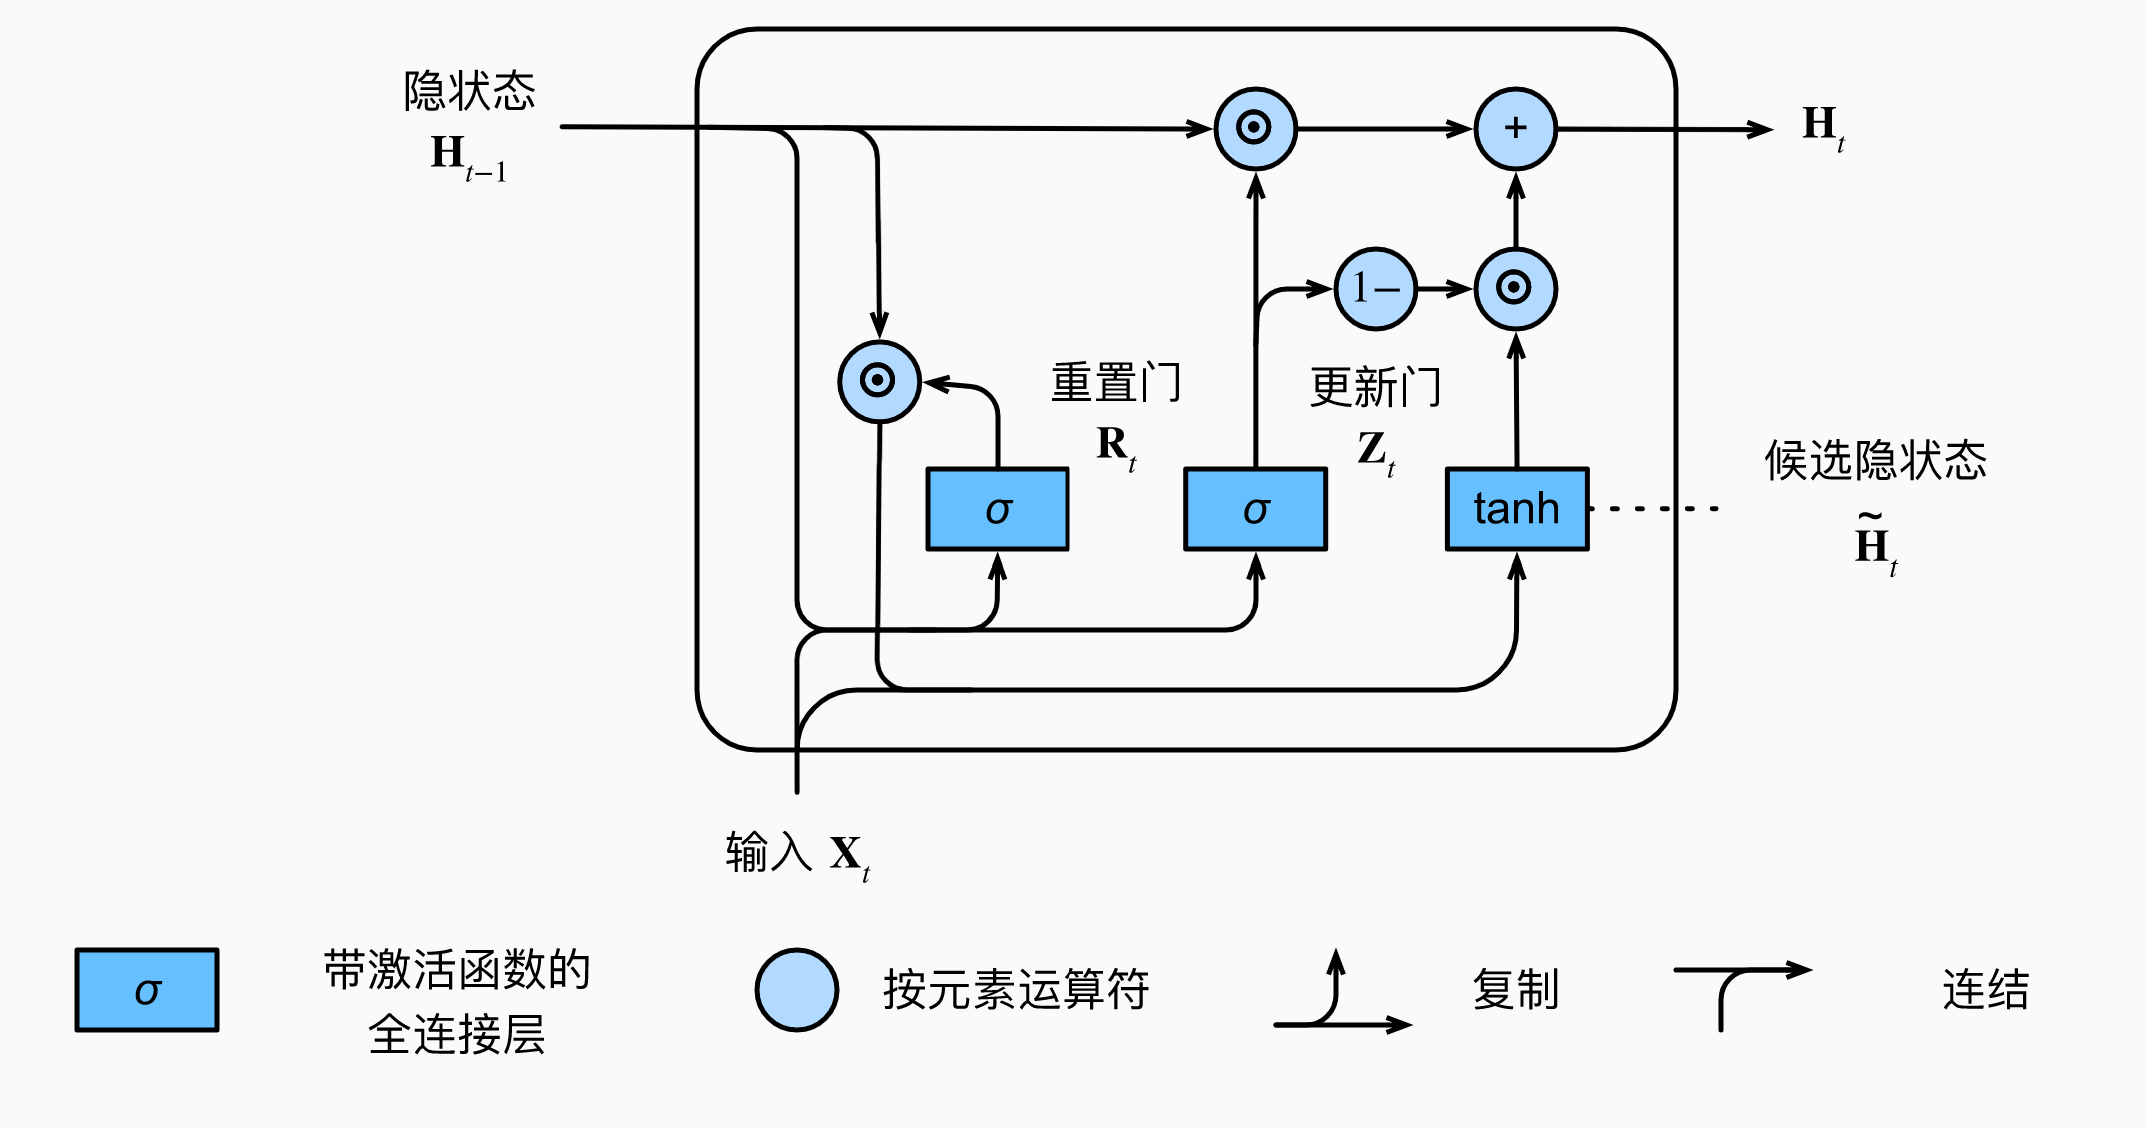
\includegraphics[width=0.8\linewidth]{pic/GRU.png}
		\caption{RNN-GRU 模型}
	\end{figure}


	整体网络结构上,GRU和LSTM大体相同,只是GRU在设计隐状态输入时采用了随机数而非上一状态首或尾部隐状态输出。

\section{实验过程}
	\subsection{数据预处理}
	\hspace{1.4em}
	在获得⼀个 Token 对应的 Embedding 时,首先尝试获取该 token 对应的 embedding 向量,获取不到则否则跳过该词。在获取句子时,只获取长度为 \textbf{maxLength} 以内的token,对于超过该部分的token,用0补齐
	
	\subsection{训练方法与模型参数}
		\subsubsection{训练方法与参数}
		
		\paragraph*{环境配置} 训练时我使用了 GPU 加速,在服务器上,117个实验跑了共计36小时左右
		\paragraph*{训练优化} 训练中我选用了 Adam 作为训练优化器,$batch\_size=16, lr =10^{-3}$,Epoch 数最大设为20,并采用了早停机制:在连续5个 Epoch 准确率没有明显提升后会强制训练过程提前结束。实验中,只有 11/117 个实验跑满了20个 Epoch,这也说明了早停机制的有效性以及最大 Epoch数设为20是比较合理的。\label{EarlyStop}
		
		\paragraph*{训练过程} 训练使用 \verb|train.txt| 中的数据作为测试集,使用 \verb|validation.txt| 作为验证集检测训练过程中准确率的变化并作为早停机制的依据,\verb|test.txt| 作为测试集评估最终模型的训练效果。每组实验的训练过程被记录在 \verb|logs/<task_name>.log| 中,整体的训练过程(包含每个模型最终的训练结果,训练时长,训练Epoch数等信息)记录在 \verb|Overall.log| 中
	
		\subsubsection{模型参数设置}
		\hspace{1.4em}
		模型定义在 \verb|models/| 文件夹下,模型参数则定义在 \verb|configs/| 文件夹下,共117组实验,编写实验参数可通过运行 \verb|config_maker/<model_name>.py| 来批量生成参数文件并运行 \verb|move_to.sh| 转移到 \verb|configs/| 文件夹下。为防止过拟合,我使用了 Dropout 机制并将 \verb|drop_keep_prob| 设为0.3,参数初始化方面,对于线性层我使用了 kaiming,xavier 或无初始化方法(上网查询资料得 pytorch 会默认调用 He-uniform 对线性层进行参数初始化),而对 LSTM 以及 GRU 层使用了正交初始化方法
		
		\paragraph*{MLP}
		\subparagraph*{参数设计} 全连接层 $hidden\_dim \in \{[512,256,128,64],[512,256,128,64,32],[512,256,128,64,32,16]\}$,以及三种不同的参数化方法共计9组实验 
		\subparagraph*{任务名} 任务命名为 \verb|MLP-h<hidden_dim>-ini_<ini method>.cfg|
		
		\paragraph*{TextCNN}
		\subparagraph*{参数设计} 卷积核尺寸 $kernel\_size \in \{[3,5],[3,5,7],[3,5,7,9]\}$,卷积核个数 $kernel\_num \in \{2,8,14,20\}$,以及三种不同的参数化方法共计36组实验 
		\subparagraph*{任务名} 任务命名为 \verb|TextCNN-ks<kernel_size>-kn<kernel_num>-ini_<ini method>.cfg|
		
		\paragraph*{RNN-LSTM}
		\subparagraph*{参数设计} 隐藏向量大小 $hidden\_size \in \{64,128,256,512\}$,LSTM层数 $num\_layers \in \{1,2,4\}$,以及三种不同的参数化方法共计36组实验 
		\subparagraph*{任务名} 任务命名为 \verb|LSTM-h<hidden_size>-l<num_layers>-ini_<ini method>.cfg|
		
		\paragraph*{RNN-GRU}
		\subparagraph*{参数设计} 隐藏向量大小 $hidden\_size \in \{64,128,256,512\}$,层数 $num\_layers \in \{1,2,4\}$,以及三种不同的参数化方法共计36组实验 
		\subparagraph*{任务名} 任务命名为 \verb|GRU-h<hidden_size>-l<num_layers>-ini_<ini method>.cfg|
		
	\subsection{结果与数据分析}
		\subsubsection{MLP}
			\textbf{实验结果}
			
			\begin{table}[h]
				\center
				\begin{tabular}{c|c|c}
					\textbf{Hidden\_dim} & \textbf{Accuracy} & \textbf{F1 score} \\
					\hline
					\textbf{[512,256,128,64]} & \textbf{0.749} & \textbf{0.785} \\
					\hline
					[512,256,128,64,32]  & 0.507 & 0.673\\
					\hline
					[512,256,128,64,32,16] & 0.507 & 0.673 \\
					
				\end{tabular}
				\caption{MLP在线性层无初始化条件下实验结果}
			\end{table}
			
			\begin{table}[h]
				\center
				\begin{tabular}{c|c|c}
					\textbf{Hidden\_dim} & \textbf{Accuracy} & \textbf{F1 score} \\
					\hline
					[512,256,128,64] & 0.797 & 0.808 \\
					\hline
					[512,256,128,64,32]  & 0.493 & 0.000\\
					\hline
					[512,256,128,64,32,16] & 0.493 & 0.000 \\
					
				\end{tabular}
				\caption{MLP在线性层 xavier 初始化条件下实验结果}
			\end{table}
		
			\begin{table}[h]
				\center
				\begin{tabular}{c|c|c}
					\textbf{Hidden\_dim} & \textbf{Accuracy} & \textbf{F1 score} \\
					\hline
					[512,256,128,64] & 0.745 & 0.770 \\
					\hline
					[512,256,128,64,32]  & 0.507 & 0.673\\
					\hline
					[512,256,128,64,32,16] & 0.507 & 0.673 \\
					
				\end{tabular}
				\caption{MLP在线性层 kaiming 初始化条件下实验结果}
			\end{table}
		\paragraph*{数据分析}
			MLP模型为其余模型的Baseline,即 $hidden\_dim \in [512,256,128,64]$,线性层无参数化情况下,$Accuray = 0.749 ,\ f1\_score = 0.785$
		\paragraph*{模型分析}
			MLP 模型优势在于模型小,速度快,实验中平均每次 MLP 模型只需2-3分钟即可跑完,这和其他模型(特别是RNN模型)形成了鲜明的对比,后者一次训练有时甚至要用到1个小时。但 MLP 模型的劣势在于能够提取到的特征实在有限,导致准确率较低,以至于 f1 score 在有些实验中会跌至0。此外,虽然参数初始化并不是 MLP 模型主要探索的,但从结果来看,xavier 初始化表现较好。
			
		\subsubsection{TextCNN}
			\textbf{实验结果}
			
			\begin{table}[h]
				\center
				\begin{tabular}{c|c|c|c}
					\textbf{Kernel\_size} & \textbf{Kernel\_num} & \textbf{Accuracy} & \textbf{F1 score} \\
					\hline
					[3,5] & 2 & 0.778 & 0.775 \\
					\hline
					[3,5] & 8 & 0.827 & 0.825\\
					\hline
					[3,5] & 14 & 0.818 & 0.816 \\
					\hline
					[3,5] & 20 & \textbf{0.840} & \textbf{0.841} \\
					\hline
					[3,5,7] & 2 & 0.740 & 0.743\\
					\hline
					[3,5,7] & 8 & 0.775 & 0.769 \\
					\hline
					[3,5,7] & 14 & 0.813 & 0.800 \\
					\hline
					[3,5,7] & 20 & 0.832 & 0.831\\
					\hline
					[3,5,7,9] & 2 & 0.832 & 0.826 \\
					\hline
					[3,5,7,9] & 8 & 0.775 & 0.786 \\
					\hline
					[3,5,7,9] & 14 & 0.793 & 0.794 \\
					\hline
					[3,5,7,9] & 20 & 0.826 & 0.832 \\
				\end{tabular}
				\caption{TextCNN 在线性层无初始化条件下实验结果}
			\end{table}
		
		
		\paragraph*{数据分析}
			TextCNN 模型相比 basline 有明显的提升,其 Accuracy 和 f1 score 分别提升了8个点和5个点。不少模型都通过了80\%大关,其中表现最好的模型为$kernel\_size = [3,5],\ kernel\_num = 20$
		\paragraph*{模型分析}
			通过仿照计算机视觉领域的 CNN 模型操作,Text-CNN在特征提取上相比普通 MLP 有了明显的提升,这是因为它可以关注到相邻词语之间的关系。从实验结果来看,总体来说卷积核个数增加对于模型性能提升有一定的帮助(只有一个例外,即第九号实验),但卷积核大小对于性能的提升没有很明显的影响,并不是卷积核设置的越多越大,性能就越好。这可能和模型本身设计有关,即 TextCNN 模型提取特征只对邻近的几个词有用,而当观测窗口扩大时并不能对更远处的词起到相同的效果,因此扩大卷积核反而会拖累性能。
			
			
		\subsubsection{RNN-LSTM}
		\textbf{实验结果}
		
		\begin{table}[h]
			\center
			\begin{tabular}{c|c|c|c}
				\textbf{Hidden\_size} & \textbf{num\_layers} & \textbf{Accuracy} & \textbf{F1 score} \\
				\hline
				64 & 1 & 0.824 & 0.818 \\
				\hline
				64 & 2 & 0.824 & 0.816\\
				\hline
				64 & 4 & \textbf{0.840} & \textbf{0.840} \\
				\hline
				128 & 1 & 0.827 & 0.819 \\
				\hline
				128 & 2 & 0.837 & 0.837\\
				\hline
				128 & 4 & 0.843 & 0.842 \\
				\hline
				256 & 1 & 0.829 & 0.826 \\
				\hline
				256 & 2 & 0.813 & 0.805\\
				\hline
				256 & 4 & 0.824 & 0.820 \\
				\hline
				512 & 1 & 0.818 & 0.810 \\
				\hline
				512 & 2 & 0.818 & 0.820 \\
				\hline
				512 & 4 & 0.493 & 0.0 \\
			\end{tabular}
			\caption{RNN-LSTM 在线性层无初始化条件下实验结果}
		\end{table}
		\paragraph*{数据分析}
			
			RNN-LSTM模型相比 baseline ,Accuracy 和 f1 score 提升了9个点和6个点,略好于 TextCNN。一个比较反常的现象是,随着参数的增加,特别是 \textbf{num\_layers} 这一参数的增加,模型性能出现了明显的下降,以至于 f1\_score 出现了跌至0的现象。出现这一现象可能有三种原因:1.训练中出现过拟合情况 2.模型过大难以训练 3.模型增大,层数增多后导致的梯度消失。通过翻阅训练记录我发现 \textbf{train\_loss} 一直停留在 0.7 左右(见下图),说明并未发生过拟合,而 \textbf{hidden\_size} 增加并不会显著降低模型性能,说明模型大小可能也不是最主要的原因,因此我推测最有可能导致这一现象的原因是随着层数增多而导致的梯度消失现象。这可能与网络结构设计有关:随着LSTM层数增加,只有最后一层的输出经过全连接层,而反向传播时梯度经过几个隐藏层后就可能会导致梯度降为0。一种可行的解决方案是取每次LSTM的输出值过MLP,或许能得到更好的性能。
			
			\begin{figure}[H]
				\centering
				\subfigure[LSTM-h512-l4-ini\_None 训练验证 Accuracy]{
					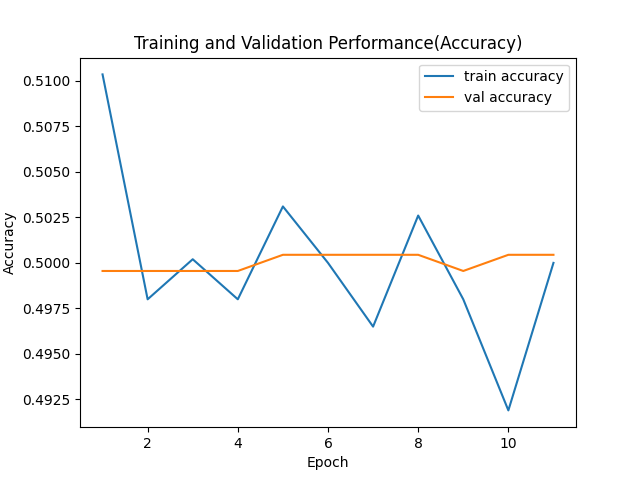
\includegraphics[scale=0.4]{pic/lstmaccuracy.png}
					
				}
				\hspace{0.2in}
				\subfigure[LSTM-h512-l4-ini\_None 训练验证 Loss]{
					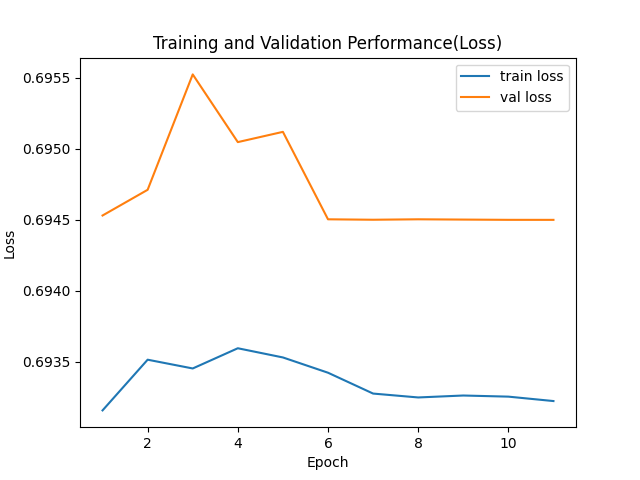
\includegraphics[scale=0.4]{pic/lstmloss.png}
					
				}
			\end{figure}
		
		\paragraph*{模型分析}
			RNN 模型的优势在于成功利用了句子的时序特征,但问题在于模型容易存在遗忘的情况,而层数增加也会带来梯度消失问题,这意味着 RNN 在模型增大时需要适当调整网络结构。此外,LSTM-RNN训练成本过高也是一个需要关注的问题,有时一次实验需要跑1到2个小时才能完成,相比TextCNN,用时几乎是后者的10倍!
		\subsubsection{RNN-GRU}
		\textbf{实验结果}
		
		\begin{table}[h]
			\center
			\begin{tabular}{c|c|c|c}
				\textbf{Hidden\_size} & \textbf{num\_layers} & \textbf{Accuracy} & \textbf{F1 score} \\
				\hline
				64 & 1 & 0.824 & 0.819 \\
				\hline
				64 & 2 & 0.848 & 0.847\\
				\hline
				64 & 4 & 0.827 & 0.824 \\
				\hline
				128 & 1 & \textbf{0.851} & \textbf{0.851} \\
				\hline
				128 & 2 & 0.832 & 0.830\\
				\hline
				128 & 4 & 0.843 & 0.846 \\
				\hline
				256 & 1 & 0.835 & 0.838 \\
				\hline
				256 & 2 & 0.843 & 0.839\\
				\hline
				256 & 4 & 0.507 & 0.673 \\
				\hline
				512 & 1 & 0.816 & 0.815 \\
				\hline
				512 & 2 & 0.827 & 0.825 \\
				\hline
				512 & 4 & 0.493 & 0.255 \\
			\end{tabular}
			\caption{RNN-GRU 在线性层无初始化条件下实验结果}
		\end{table}
		\paragraph*{数据分析}
		RNN-GRU 模型相比 RNN-LSTM 有一定的提升,在两项指标上均提高了1个点左右,而在参数增加导致性能下降这一点上二者也十分一致,甚至 RNN-GRU 模型更甚,分析其原因可能和 LSTM 相似,都是因为层数过多导致的梯度消失。
		\paragraph*{模型分析}
		作为 LSTM 模型的一个变种,GRU-RNN 模型通过调整单元结构获得了性能上的提升,得到了所有模型中最好的结果。但依然没有解决参数过多导致性能下降以及训练用时过长的问题。
	\subsubsection{参数初始化}\label{ini}
		\hspace{1.4em}
		为了探究参数初始化对模型性能肯能带来的影响,对于实验中的每一组模型参数,我都用三种不同参数初始化方法进行训练,下表为各个模型性能最佳条件下不同初始化条件的表现对比
		\begin{table}[h]
			\center
			\begin{tabular}{c|ccc}
				\textbf{Modal} & \textbf{Default} & \textbf{Xavier} & \textbf{Kaiming} \\
				\hline
				MLP & 0.749 & \textbf{0.797} & 0.745 \\
				\hline
				TextCNN & 0.818 & 0.816 & \textbf{0.821}\\
				\hline
				RNN-LSTM & 0.840 & \textbf{0.848} & 0.840 \\
				\hline
				RNN-GRU & 0.827 & 0.832 & \textbf{0.837} \\
			\end{tabular}
			\caption{四种模型在不同初始化条件下的准确率}
		\end{table}
		\begin{table}[h]
			\center
			\begin{tabular}{c|ccc}
				\textbf{Modal} & \textbf{Default} & \textbf{Xavier} & \textbf{Kaiming} \\
				\hline
				MLP & 0.785 & \textbf{0.808} & 0.770 \\
				\hline
				TextCNN & 0.816 & 0.810 & \textbf{0.822}\\
				\hline
				RNN-LSTM & 0.840 & \textbf{0.845} & 0.840 \\
				\hline
				RNN-GRU & 0.824 & 0.828 & \textbf{0.836} \\
			\end{tabular}
			\caption{四种模型在不同初始化条件下的 F1 score}
		\end{table}
		实验表明多数情况下,特定参数初始化条件能将模型性能提升0.5到1个点,其中MLP模型的准确率甚至整整提升了5个点之多!另外一个值得注意的点是仅从实验结果来看,似乎 Xavier 和 Kaiming 没有明显的优劣之分,这和之前搜索资料中提到的 Kaiming 方法更适合 RELU 激活函数有所不同。 
\section{思考与讨论}
\subsection{何时终止训练?}
	\hspace{1.4em}
	在本实验中,我采用了早停机制(详见\ref{EarlyStop}),有91\%的实验于任务结束前终止。起到了减少训练时间和在一定程度上避免过拟合的作用。
	
	然而仔细思考,如此设计也会存在一定的问题,首先是验证的过程本身可能带来一定的时间开销,本次实验中由于验证方式相对容易因此没有关注这个问题,但在其它一些实验中过于频繁的验证可能会拖累训练速度。
	
	另一个更重要的问题是,有时只通过验证集并不能发现所有的问题,比如在此前在 RNN 模型中出现过的参数过大导致性能下降问题中,如果能够尽早发现 $train\_loss$ 停留在了一个异常的位置而停止训练,就可以避免后续的不必要训练,考虑到单次LSTM训练成本高达1个多小时,这种方式可以解决的时间成本十分可观
\subsection{参数初始化}
	\hspace{1.4em}
	在\ref{ini} 中曾展示过不同参数初始化对模型性能的影响,总体来看,参数初始化对模型性能提升有一定的作用,而不同的模块也有适合自己的模块的初始化方法,如RNN中的循环单元比较适合用正交初始化,但也有一些模块中的最优初始化并不总是唯一确定的,比如在不同的模型中线性层最佳初始化方式就不尽相同。作为一种训练技巧,参数初始化的选择也需要根据具体的问题具体分析,找到最佳的初始化方法。
\subsection{如何避免过拟合?}
	\begin{itemize}
		\item 如本部分第一节所讨论的那样,通过调整训练中的监督策略,通过每一次迭代后训练集和验证机的表现来判断是否出现了过拟合情况并即使终止训练
		\item 调整 dropout 值,让每一层网络“忘掉”更多东西
		\item 使用更大的训练集,提高模型的泛化能力
	\end{itemize}
\subsection{不同模型的比较与选择}
	\hspace{1.4em}
	从最终结果来看,RNN-GRU 模型在性能上拔得头筹,但RNN模型又存在的参数增加导致性能降低以及训练时间成本过高的问题,TextCNN 虽然在性能上略弱(实际上只落后1个点),但其较短的训练时长以及相对简单的网络结构使其更受人亲睐。
	\hspace{1.4em}
	不过目前看来 TextCNN 性能提升随着模型增大也存在一定的瓶颈,倘若 RNN 通过调整网络结构(如引入类似resNet的结构)或使用更好的训练方法,相信一定能在性能上表现出更大的优势。
\section{总结}
	\hspace{1.4em}
	本次实验中,我实现了 MLP, TextCNN, RNN-LSTM, RNN-GRU 四种模型,选取不同的参数进行实验,\textbf{最终得到的最高准确率为 85.1\%,最高 F1 score 为 0.851}.实验中我搭建了具有可扩展性的代码框架,比较了不同参数下模型性能的表现,并横向对比的不同模型,分析他们各自的优势与不足。针对实验中出现的问题,我提出了自己的猜测,并给出了可能的解决方法。
	本次实验是我第一次真正上手神经网络框架。通过本次实验我更加熟练地掌握了 pytroch 编程框架以及其它 python 包的使用,并对机器学习训练的过程(从清洗数据到建立模型再到配置实验最后再到数据分析)有了更清晰的体会和认识。
	受限于时间和设备性能,本次实验探究止步于此,未来可能还可以进一步探究的点有
	\begin{itemize}
		\item 尝试引入更多模型框架,如Transformer 模型的 Attention 机制
		\item 探索更多的训练优化技巧,如使用 SGD 代替 ADAM,前者相比后者可以更好地避免掉入局部最优陷阱。再如可以探究更多的参数初始化技巧。
		\item 可以尝试引入更多的词向量模型,如 BERT 等,将更多的词义融合到 Embedding 中
	\end{itemize}
\section{附录}
	\subsection{项目结构}
		\begin{lstlisting}
		{
		|-config_maker: 训练参数设置文件生成器
		|-configs: 所有训练参数文件
		|-data: 训练集、测试集、验证集
		|-logs: 训练日志,Overall记录的是整体训练情况
		|-model: 模型定义文件
		|-tools
			|- trainer.py: 训练工具
			|- logger.py: 日志记录工具
		|-README.md: 项目说明文件
		
		}
		\end{lstlisting}
	\subsection{代码运行说明}
	\hspace{1.4em}
		运行本项目需要安装pytorch,numpy,pathlib,gensim,json 等库。配置好环境后,运行 \verb|python main.py -cf=<task\_name>| 即可运行实验,如果不指定配置文件则默认对 \verb|configs| 下所有文件进行实验。
		运行 \verb|config_maker/<model_name>.py| 可批量生成配置文件
	
% End edit to here
%%%%%%%%%%%%%%%%%%%%%%%%%%%%%%%%%%%%%%%%%%%%%%%%%%%%%%%%%%%%%

\end{spacing}
\end{document}

%%%%%%%%%%%%%%%%%%%%%%%%%%%%%%%%%%%%%%%%%%%%%%%%%%%%%%%%%%%%%
